\documentclass[a4paper,11pt]{article}%
    
\usepackage{fullpage}%
\usepackage[T1]{fontenc}%
\usepackage[utf8]{inputenc}%
\usepackage[francais]{babel}% % Adjust the main language

\usepackage{graphicx}%
\usepackage{url}%
\usepackage{abstract}%

\usepackage{mathpazo}%

\usepackage{listings}%

\usepackage{subcaption}

\parskip=0.5\baselineskip

\sloppy

\begin{document}

\title{Activités, problèmes, résultats}

\author{Clément Legrand-Lixon}

\date{}

\maketitle

\paragraph*{22 Mai 2018}

Arrivée dans le laboratoire (Cristal). Rencontre de l'équipe (doctorants et stagiaires). Installation du poste de travail (Ubuntu, espace de travail : VSC, latex, R). Découverte du problème, recherche d'informations (variantes: multi-dépôts, avec capacité, avec limite de temps...). Lecture des articles \emph{A new enhancement of the Clarke and Wright savings heuristic for the capacitated vehicle routing problem} (K. Altınel, T. Oncan), et \emph{A simple, deterministic, and efficient knowledge-driven heuristic
for the vehicle routing problem} (Florian Arnold, Kenneth Sorensen). Vu administration pour la gratification de stage. 

\paragraph*{23 Mai 2018}

Fin de lecture des articles, résumé des articles tapés en tex. Implémentation de l'algorithme de Clarke and Wright (C W), en python.
Mise en place d'une heuristique basique (avec paramètre $\lambda$). 
Tests de l'algo sur des instances fabriquées aléatoirement. 
Tentative pour trouver une valeur optimale pour le paramètre selon la taille de l'entrée. 
Résultats disponibles avec la figure \ref{lambda}.

\begin{figure}[ht]
	\centering
	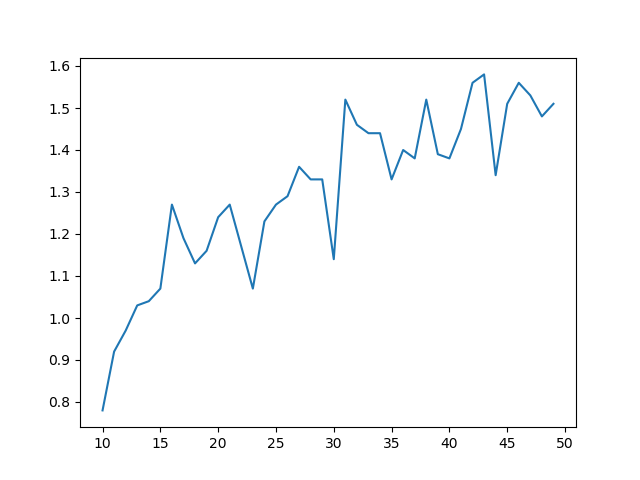
\includegraphics[width=0.7\textwidth]{best_lambda.png}
	\caption{Valeur de lambda optimale}
	\label{lambda}
\end{figure}

\paragraph*{24 Mai 2018}

Rencontre avec encadrante senior : Marie-Éléonore, bilan sur les premiers jours. Obtention du code C++ de l'heuristique de CW (complète, mais quelques erreurs présentes à corriger). 
\underline{Objectif}: Pour la semaine prochaine, faire une présentation reprenant la nouvelle heuristique développée dans l'article de F. Arnold et K. Sorensen. 
Et éventuellement implémentation des opérateurs locaux utilisés dans l'heuristique en expliquant les intérêts et limites de chaque (complexité, avantage...).  
Début de la présentation. Recherche d'articles détaillant les opérateurs utilisés. Peu de résultats (page wikipédia pour Lin Kernighan). 

\paragraph*{25 Mai 2018}

Rencontre avec Lætitia Jourdan (responsable de l'équipe). Implémentation de l'heuristique de Lin-Kernighan : pour une tournée donnée, optimise la visite des clients (utilisée pour TSP). Commence par réaliser 2-opt (cherche un changement entre deux arêtes qui améliore la tournée). Si trouvé on passe 3-opt (echange de 3 aretes), jusqu'à k-opt (k choisi). Puis applique la meilleure modif (la meilleure i-opt). S'arête lorsque plus d'améliorations possibles). 

Implémentation de 2-opt en python, tests sur quelques instances. On part de \ref{test1}, et en appliquant 2-opt on obtient \ref{test1_2opt}. 'Dépôt représenté en bleu). 

\begin{figure}[ht]
	\centering
	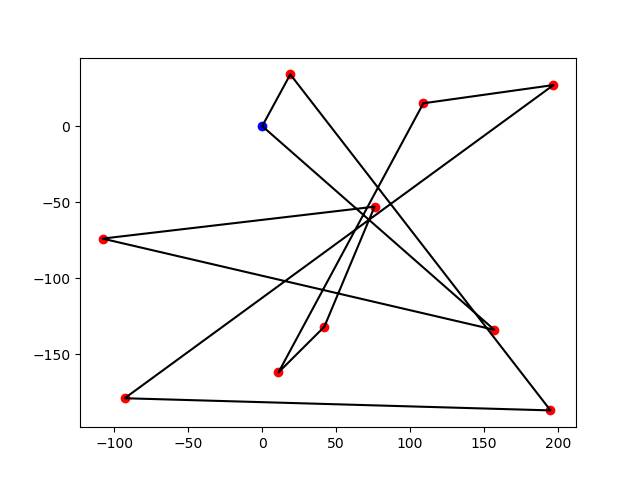
\includegraphics[width=0.5\textwidth]{test1_init.png}
	\caption{Instance initiale}
	\label{test1}
\end{figure}

\begin{figure}[ht]
	\centering
	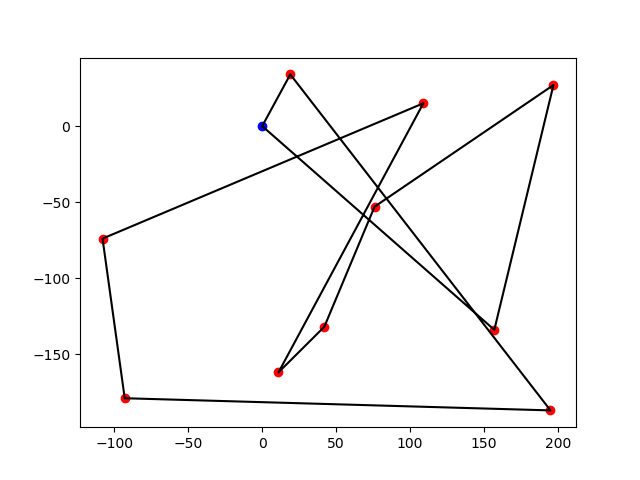
\includegraphics[width=0.5\textwidth]{test1_2opt.png}
	\caption{Optimisation avec 2-opt}
	\label{test1_2opt}
\end{figure}

Rencontre de problèmes avec des instances supérieures, et LK. $\rightarrow$ A résoudre lundi. Opérateur à utiliser principalement sur des petites portions de route, complexité élevée $O(n^k)$ avec $n$ le nombre de clients. 

\paragraph*{28 Mai 2018}

\underline{Objectifs} : finir d'implémenter LK, tester, et finir le développement dans la présentation. Améliorer présentation. Implémenter un autre opérateur \emph{Cross-exchange} ou \emph{Ejection-chain}.

\underline{Réalisation} :  LK corrigé (fonctionne avec 2-opt... généraliser à k-opt ?). Tests réalisés sur la tournée en image \ref{test4_20_init}, où on obtient la tournée en image \ref{test4_20_LKopt}.

\begin{figure}[ht]
\centering
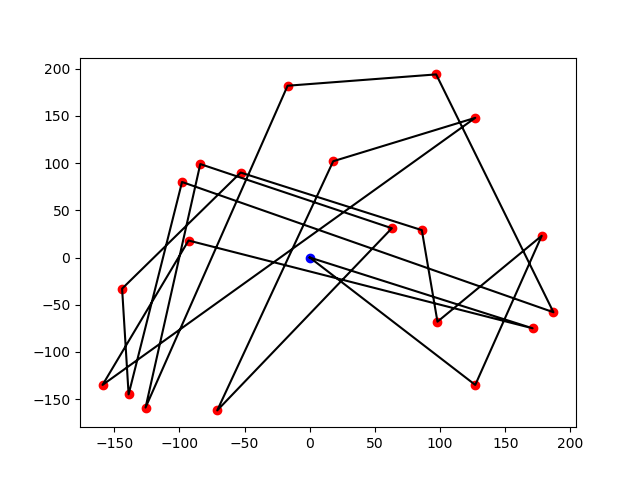
\includegraphics[width=0.5\textwidth]{test4_20_init.png}
	\caption{Instance initiale pour $20$ clients}
	\label{test4_20_init}
\end{figure}

\begin{figure}[ht]
\centering
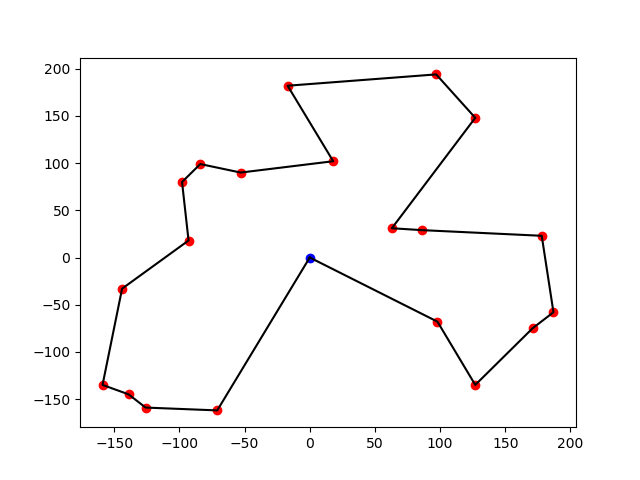
\includegraphics[width=0.5\textwidth]{test4_20_LKopt.png}
	\caption{Solution obtenue avec Lin-Kernighan}	\label{test4_20_LKopt}
\end{figure}

Création (enfin !) d'un dépôt GIT, pour partager mes documents (travail, présentations...)

Début implémentation de Cross-exchange (local). Article détaillant cet opérateur : \emph{A Tabu Search Heuristic for the Vehicle Routing Problem with Soft Time Windows}. Cet opérateur consiste en l'échange de toute séquence de clients entre 2 tournées. L'aspect local est d'autant plus intéressant, que la complexité passe en quadratique dans le pire cas, au lieu de $O(n^4)$. 
On commence par calculer $k$ pp voisins pour chaque nœud (pré-calcul). Après avoir choisi une arête $(a,b)$, on regarde les plus proches voisins du premier nœud, on prend le premier qui est sur une tournée différente, $(c,v_a)$. 
On construit les deux arêtes $(a,v_a)$ et $(c,b)$. Puis on essaye d'échanger $(v_a+1, v_a+2)$, avec $(b+1,b+2)$, ou $(b+2,b+3)$ ainsi de suite jusqu'à retomber sur l'arête de départ ou trouver une amélioration. 
En pratique on trouve rapidement une amélioration d'où une complexité en général linéaire. 
Il faut aussi veiller à ne pas dépasser les contraintes de capacité (non prises en compte dans un premier temps). 
Fin implémentation, tests réalisés sur une instance particulière (cf ...), 3 exécutions ont été réalisées sur des arêtes différentes, (arête choisie en rouge). Exemple avec l'image \ref{test1CE_init}, on obtient le résultat sur l'image \ref{test1CE_imp}. 

\begin{figure}[ht]
\centering
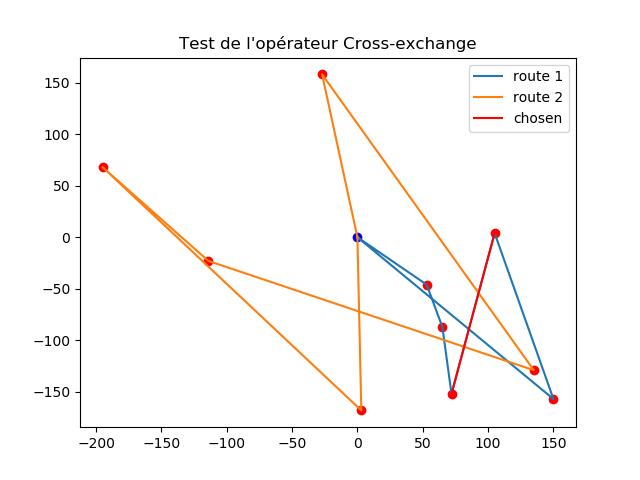
\includegraphics[width=0.5\textwidth]{test1CE_init.png}
	\caption{Instance initiale pour $10$ clients répartis sur 2 tournées}
	\label{test1CE_init}
\end{figure}

\begin{figure}[ht]
\centering
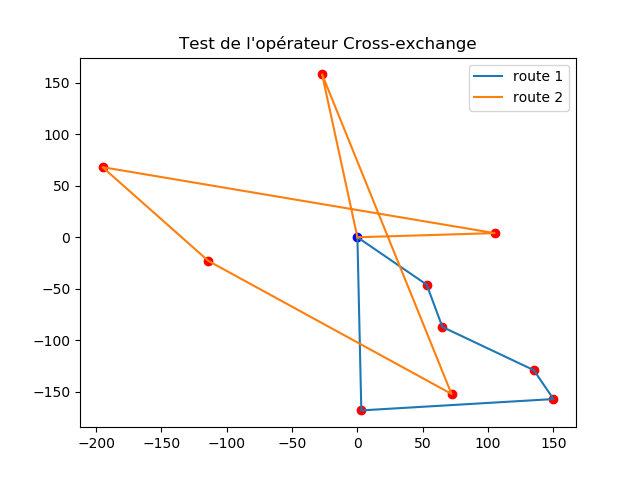
\includegraphics[width=0.5\textwidth]{test1CE_imp.png}
	\caption{Amélioration obtenue avec Cross-exchange}	
	\label{test1CE_imp}
\end{figure}

\paragraph*{29 Mai 2018}

\underline{Objectifs} : Corriger présentation pour cross-exchange. Faire implémentation de ejection-chain, tester. Finir présentation ? Finir de corriger code C++ ?

\underline{Réalisation} : Ajout de cross-exchange dans la présentation. Implémentation de l'ejection-chain, reste quelques problèmes (ajout/suppression de routes, manque les capacités). Ajout des capacités pour le cross-exchange, et découverte problème dans implémentation $\rightarrow$ correction et nouveaux tests. Epuration code et homogénéisation des notations. Commentaires ajoutés. Tests pour correction de CE (et ajout de capacités): 

\begin{figure}[ht]
\centering
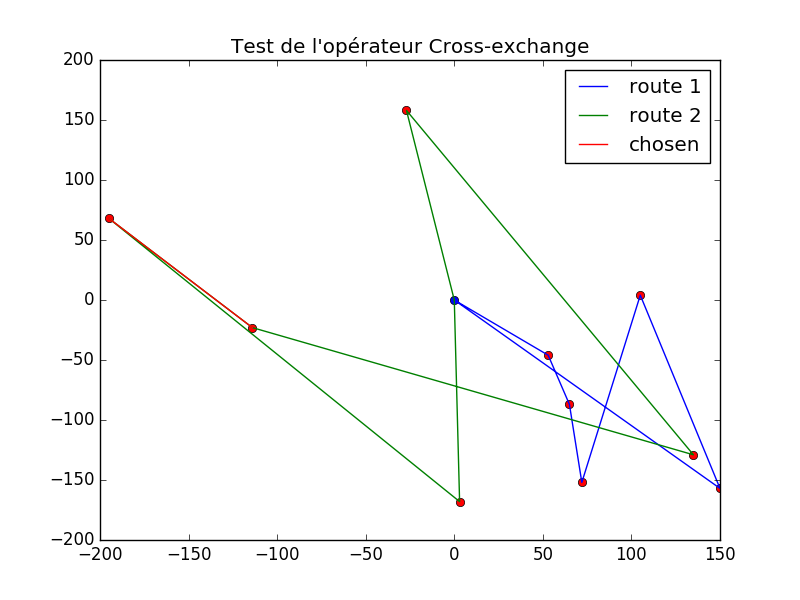
\includegraphics[width=0.5\textwidth]{test2CE_init.png}
	\caption{Instance initiale pour $10$ clients répartis sur 2 tournées}
	\label{test2CE_init}
\end{figure}

\begin{figure}[ht]
\centering
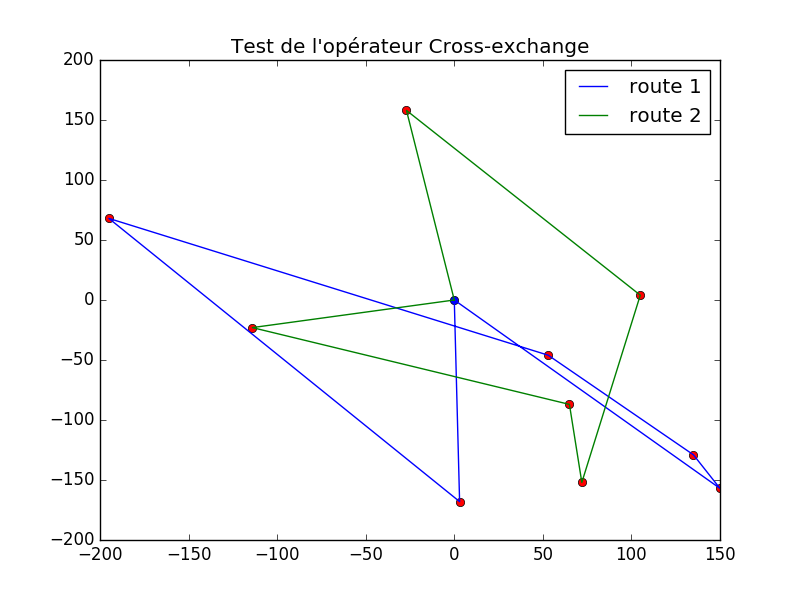
\includegraphics[width=0.5\textwidth]{test2CE_imp.png}
	\caption{Amélioration obtenue avec Cross-exchange}	
	\label{test2CE_imp}
\end{figure}

Tests pour ejection-chain (sans capacités): initialement avec image \ref{test1EC_init}, pour obtenir l'image \ref{test1EC_imp} (21 clients, 3 routes, 15 replacements).

\begin{figure}[ht]
\centering
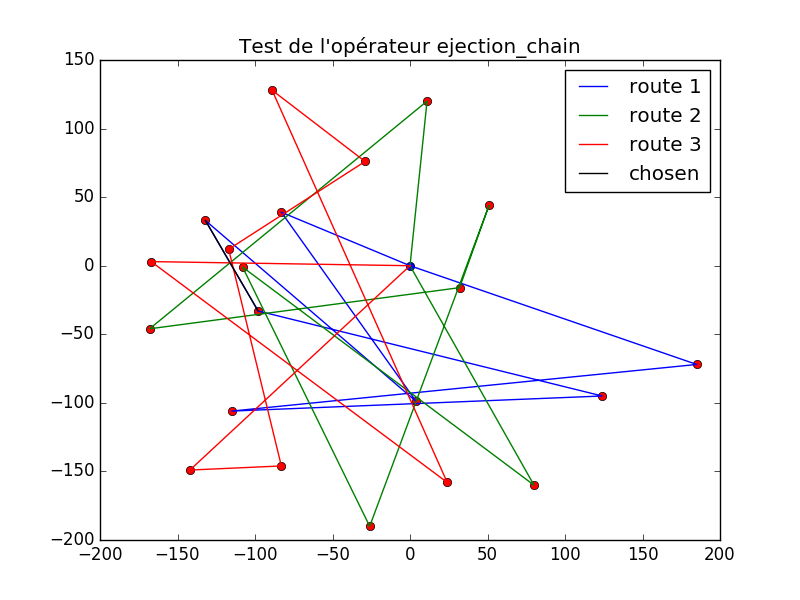
\includegraphics[width=0.5\textwidth]{test1EC_init.png}
	\caption{Instance initiale pour $21$ clients répartis sur 3 tournées}
	\label{test1EC_init}
\end{figure}

\begin{figure}[ht]
\centering
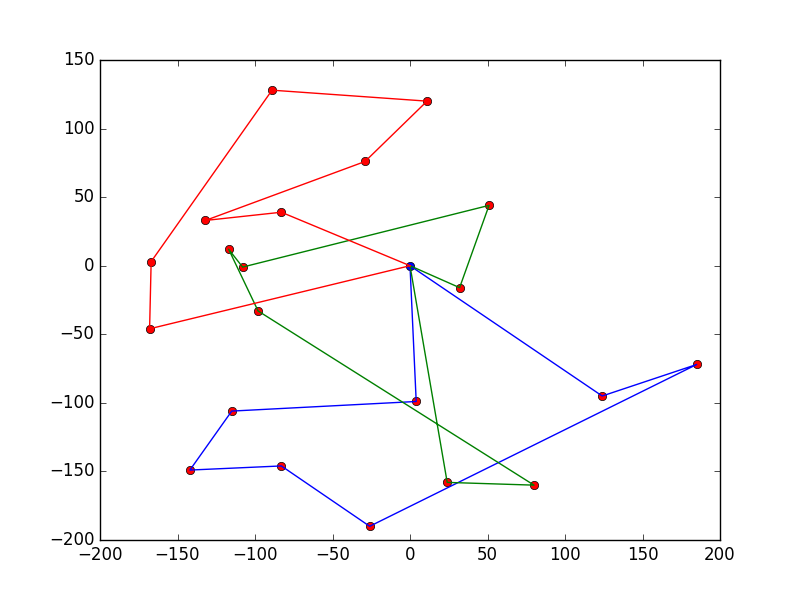
\includegraphics[width=0.5\textwidth]{test1EC_imp.png}
	\caption{Amélioration obtenue avec Ejection-chain (15 replacements)}
	\label{test1EC_imp}
\end{figure}

\paragraph*{30 Mai 2018}

Fin implémentation ejection-chain (avec gestion de capacité), \underline{création et suppression de route à faire}. Ajout à la présentation, et fin (?) de celle-ci. Re-correction du cross-exchange (et cette fois c'est bon!, les clients échangés initialement n'étaient pas bons). Article pour ejection-chain dans vrp with time-window: \emph{Fast Ejection Chain Algorithms for
Vehicle Routing with Time Windows} de Herman Sontrop, Pieter van der Horn, and Marc Uetz.
Regroupement des opérateurs, et début implémentation de l'heuristique (fonction de pénalisation, recuperation de la pire arête, execution des opérateurs). Premier test (beaucoup d'erreurs...). Correction, principal problème : opérateurs pas utilisables si beaucoup de tournées (CE, n'est censé géré que 2 tournées...). 

\paragraph*{31 Mai 2018}

Correction heuristique, ajout de l'optimisation globale, reset et update des fonctions de pénalisation. Tests sur différentes instances avec capacité totale variable. Premiers tests plutôt concluants, calcul assez rapide (30 sec pour 100 clients). Résultats présents sur les images \ref{test2_Heu_init} et \ref{test2_Heu_imp}. 

\begin{figure}[ht]
\centering
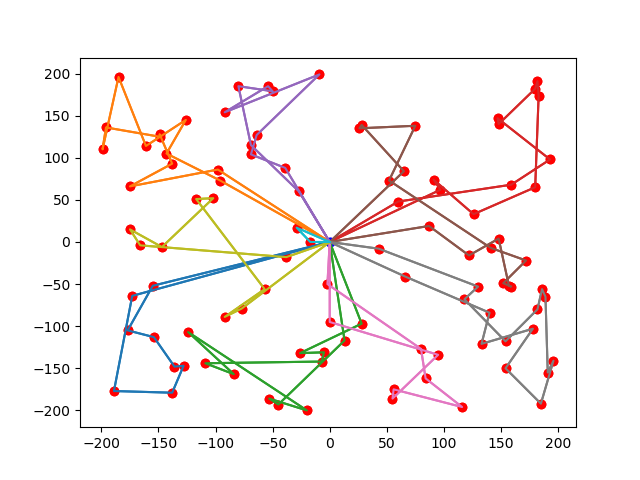
\includegraphics[width=0.5\textwidth]{test2_heuristic_init.png}
	\caption{Instance initiale pour 100 clients, avec Clark and Wright}
	\label{test2_Heu_init}
\end{figure}

\begin{figure}[ht]
\centering
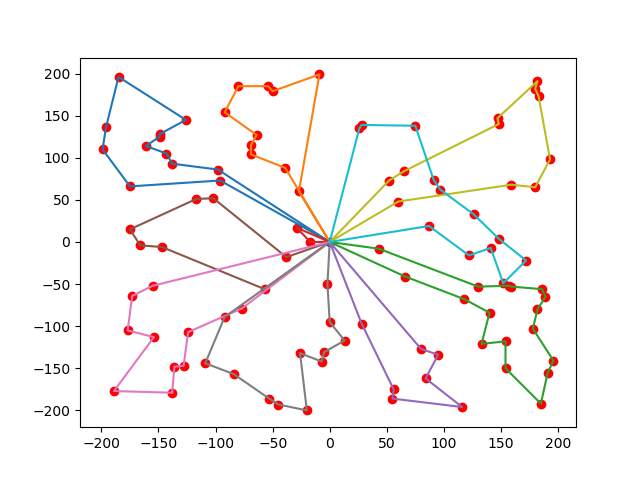
\includegraphics[width=0.5\textwidth]{test2_heuristic_res.png}
	\caption{Amélioration obtenue avec l'heuristique}
	\label{test2_Heu_imp}
\end{figure}


Remarques: toujours quelques erreurs au niveau du dépôt à cause de LK (par ailleurs qui se contente de 2-opt, à voir s'il est utile d'aller plus loin). Actuellement, l'heuristique ne choisit que des solutions améliorantes, il est possible de passer à côtés de grosses optimisations (ou alors capacités trop restrictives...).  


\underline{Conférence, Blockchains et Cryptomonnaies, par Jean-Paul Delahaye}: Présentation des notions (utilisation des Blockchains, développement sur les crypto-monnaies). Limites et future.
Principales notes:
\begin{itemize}
\item Blockchain: fichier multiplié sur un réseau P2P (donc indestructible). On peut écrire dessus en respectant des contraintes définies sur le réseau.
\item Cryptomonnaies (ou crypto-actif $\rightarrow$ pas vraiment une monnaie à cause de sa volatilité).
\item Pour ajouter une page au blockchain du bitcoin (justification de transaction), il faut inverser partiellement une fonction de hash, pour que la page ajoutée ait la bonne signature. Contrainte sur la taille de la page 1 MO (suscite un fork en 2017 $\rightarrow$ division bitcoin et bitcoin cash). Preuve d'intérêt: toutes les 10 min un certain nb de bitcoins sont attribués (jusque 2140) à ceux qui ont trouvé la solution. Difficulté ajustée si + ou - de 10 min en moyenne, de sorte à ce que la puissance de calcul nécessaire soit toujours plus importante. 
\item Aujourd'hui minage = 3 centrales nucléaires (dont la puissance principale est en Chine). Cette quantité démentielle d'electricité pose problème. (il faut effectuer de l'ordre de $10^{18}$ calculs pour miner le bitcoin en 10 min.

\item Ces monnaies (même toutes réunies) ne peuvent concurrencer l'or sur le marché financier (8000 milliards de dollars pour l'or contre 300 milliards pour les crypto-actifs).

\item D'autres crypto-monnaies voient le jour, moins énergivores : preuve d'enjeu.

\item Vulnérabilités possibles (prédiction Adi Shamir): attaques sur les courbes elliptiques, ou fonctions de hash; attaque à 51\%, qqun possède plus de la moitié de la puissance de calcul du réseau. 

\item Pas assez de transactions par seconde (environ 4/s), pour etre adapté au marché financier (comme Paypal). 
\end{itemize}

\underline{Bilan réunion}: Ajout/supp de routes inutiles à priori pour ce qu'on veut faire. Améliorer l'algo CW (au moins un 2 opt supp). Retravailler la partie sur la pire arête dans l'article. Utiliser les instances de la littérature pour les tests. Objectif principal semaine prochaine : trouver (?) un lien entre solutions améliorées et solutions CW.

\paragraph*{1 Juin 2018}

Amélioration de l'heuristique en retravaillant EC, maintenant parcours de l'espace de solutions autour d'une solution globale tant qu'on trouve pas mieux (EC plus flexible). Evaluation de l'amélioration (cf tableau sur brouillon). Amélioration de la solution initiale, et comparaison entre celle-ci et solution obtenue avec l'heuristique. Besoin de refactoriser le code et de l'alléger, modifications pas toujours claires...

\paragraph*{4 Juin 2018}
Réunion d'équipe le matin de 10 à 12. Prochaine réunion le 4 Juillet.

Amélioration de l'heuristique (correction de problèmes et ajout de fonctionnalités : regroupement de routes à la fin si la route ne contient qu'un client, correction de LK). 
Tests effectués sur des instances de la littérature (gestion de fichier xml). Résultats bons par rapport à ce qui est attendu: par exemple pour l'instance $A-n32-k05$, on part initialement du résultat en image \ref{initial_An32k05}, pour arriver à la solution en image \ref{solution_An32k05} grâce à l'heuristique programmée. Pour comparer les solutions de départ et d'arrivée, on affiche les arêtes communes entre ces solutions, ce que l'on peut voir en image \ref{edges_An32k05}. Analyse des arêtes communes entre les solutions de départ et d'arrivée. Lien avec enveloppe convexe, triangulation de delaunay ? 

\begin{figure}[ht]
\centering
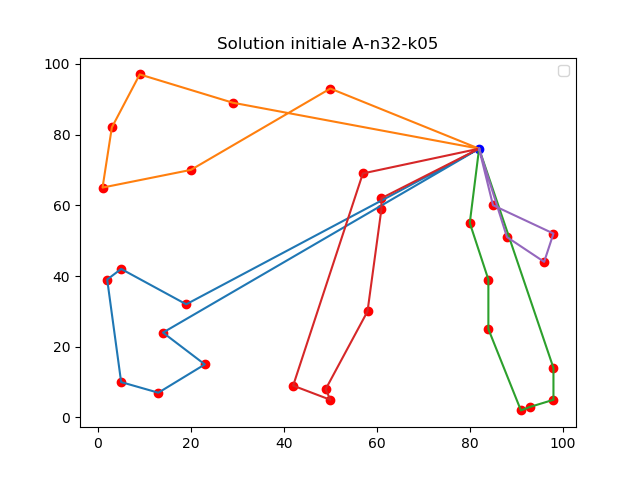
\includegraphics[width=0.5\textwidth]{initial_An32k05.png}
	\caption{Solution initiale de l'instance $A-n32-k05$, avec Clark and Wright}
	\label{initial_An32k05}
\end{figure}

\begin{figure}[ht]
\centering
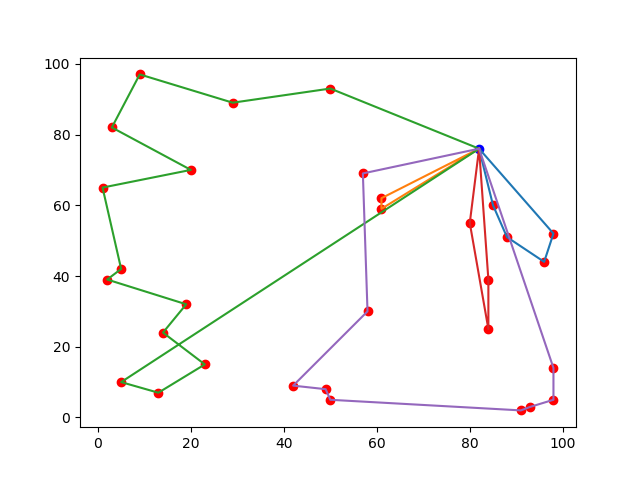
\includegraphics[width=0.5\textwidth]{solution_An32k05.png}
	\caption{Solution obtenue avec l'heuristique sur l'instance $A-n32-k05$}
	\label{solution_An32k05}
\end{figure}

\begin{figure}[ht]
\centering
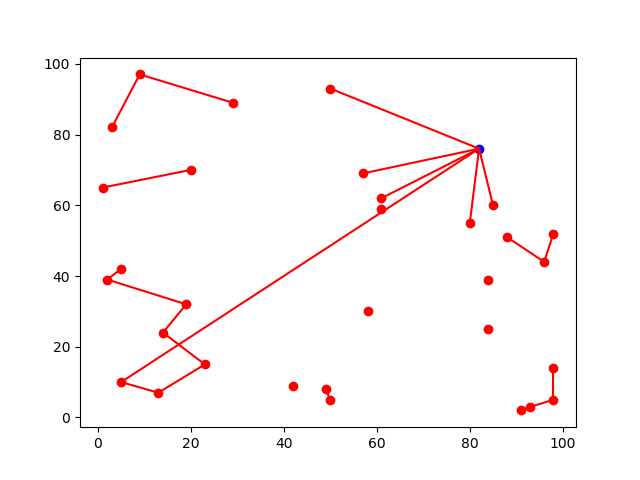
\includegraphics[width=0.5\textwidth]{commonEdges_An32k05.png}
	\caption{Arêtes communes entre la solution initiale et la solution obtenue avec l'heuristique}
	\label{edges_An32k05}
\end{figure}

\paragraph*{5 Juin 2018}
Correction d'une erreur détectée dans l'heuristique (gestion des capacités). Ajout de plusieurs instances (une dizaine). Tentatives pour trouver des liens entre les arêtes; utiliser les métriques définies pour l'heuristique.

\paragraph*{6 Juin 2018}
Amélioration code, modification paramètre. Tests des métriques (profondeur, largeur, coût), et classement selon le rang. Quelques propriétés peut-être intéressantes (cf présentation des résultats).

\paragraph*{7 Juin 2018}

\underline{Réunion}: présentation des résultats obtenus au cours de la semaine. Discussion sur l'heuristique, et les résultats (normal que la meilleure solution initiale ne donne pas la best via l'heuristique). Présentation résultats sur la conservation des arêtes. 

\underline{Objectifs}: pour la semaine prochaine:
\begin{itemize}
\item Stochastisation de l'heuristique (avec 2 opt et CE pour commencer)
\item Faire tourner l'algo sur des paramètres autour des valeurs utilisées dans l'article
\item Tableau pour présenter les résultats (paramètres choisis, moyenne des res, best, distance de la best à l'opt selon une métrique à définir).
\end{itemize}

Amélioration de CW (prise en compte des trois paramètres cf article de Altmel/Ontcan). Test de l'heuristique sur toutes les valeurs possibles ($\lambda$ : $0.1 - 2$, $\mu$ : $0 - 2$, $\nu$ : $0 - 2$). Très long... Résultats pour $1500$ tours. 

\paragraph*{8 Juin 2018}

Choix d'un pivot aléatoire dans l'opérateur Cross-exchange: permet un parcours plus large de l'ensemble des solutions. Tests effectuées pour regarder l'influence de certains paramètres (times et gs). Choix de prendre $times = 1500$ pour compromis résultats-temps, et $gs = 10$ car meilleurs résultats. Tous les tests qui suivent seront effectuées sur l'instance A-n37-k06. Ecriture des résultats au fur et à mesure dans un fichier (results.txt conservé dans un dossier portant le nom de l'instance). Le résultat est en moyenne inférieur au résultat de l'heuristique déterministe. Calcul pour des valeurs (lam,mu,nu) différentes. 

\paragraph*{11 Juin 2018}
On continue les tests sur les deux heuristiques. Résultats placés dans des fichiers (determinists.txt et stochastics.txt), l'heuristique deterministe renvoie un meilleur résultat que l'heuristique stochastique, en testant pour toutes les valeurs possibles de lam,mu,nu. 

Etude de la conservation des arêtes, en partant de la meilleure solution initiale, environ la moitié des arêtes sont conservées par rapport à la meilleure solution connue. Ajout de la conservation d'arêtes dans l'heuristique. Plusieurs idées pour les choisir: 
\begin{itemize}
\item Aléatoirement (a)
\item Garder celles qui sont rattachées au dépôt (r)
\item Par apprentissage (l)
\end{itemize}
\underline{Comment utiliser ces arêtes ?}
2 idées:
\begin{itemize}
\item Les arêtes choisies ne sont pas touchées lors des opérations locales et l'algo suit son cours. Les arêtes choisies peuvent réinitialisées si on trouve une meilleure solution. (C)
\item Les arêtes qui ne sont pas choisies sont supprimées (création de nouvelles tournées). On essaie de construire une meilleure solution à partir de là. (D)
\end{itemize}

Pour l'instant seules ont été implémentées les versions C-a-(d,s) et C-r-(d,s). Tests: peu concluants, amélioration par au déterministe et au stochastique sur quelques SI.

\paragraph*{12 Juin 2018}
 Implémentation heuristique D versions déterministes et stochastiques. Description de la méthode:
 \begin{itemize}
 \item On fait CW
 \item On commence par déterminer des arêtes à conserver
 \item On élimine les autres 
 \item On reconstruit les morceaux de tournée en rattachant toutes les extrémités au dépôt
 \item On applique de nouveau CW (choix des paramètres ?, on divise tout par 2, on prend les meilleurs paramètres)
 \item On applique l'heuristique normalement
\end{itemize}

Au final on a 2 algos qui travaillent sur les arêtes communes. Un qui conserve les arêtes choisies, et essaie d'améliorer la solution. Les arêtes à conserver sont modifiées aléatoirement si une nouvelle solution est trouvée, ou lorsqu'on réinitialise la solution courante (meilleurs résultats de cette manière). 
L'autre méthode, détruit les arêtes que l'on ne veut pas conserver et reconstruit une nouvelle solution en s'appuyant sur les arêtes conservées. Cette méthode est d'autant plus efficace que les arêtes choisies sont optimales, et que la solution initiale a de nombreuses arêtes en commun avec la solution optimale.
Ces deux algos ont une variante au niveau du CE (soit déterministe, soit stochastique).
\paragraph*{13 Juin 2018}
Divers tests pour préparer la réunion. Récup d'images. Présentation.
 

\end{document}